
% Lecture Template for ME3001-001-Tristan Hill - Spring 2017 - Fall 2017 - Fall 2020
% Mechanical Engineering Analysis with MATLAB
% Module 2 - Non-Linear Equations
% Topic 5 - A Mechanical Design Problem

% Document settings

%\documentclass{beamer}                  % for presentation ?
\documentclass[handout]{beamer}  % for handout ?
\usepackage{/home/thill/Documents/lectures/analysis_lectures/analysis_lectures}

\newcommand{\MNUM}{2\hspace{2mm}} % Module number
\newcommand{\TNUM}{5\hspace{2mm}} % Topic number 
\newcommand{\moduletitle}{Non-Linear Equations} % Titles and Stuff
\newcommand{\topictitle}{Mechanical Design Problem} 

\newcommand{\sectiontitleI}{Problem Statement} % More Titles and Stuff
\newcommand{\sectiontitleII}{Mathematical Model}
\newcommand{\sectiontitleIII}{Solution Approach}
\newcommand{\sectiontitleIV}{Design!}

\newcommand{\btVFill}{\vskip0pt plus 1filll}

% custom box
\newsavebox{\mybox}

\author{ME3001 - Mechanical Engineering Analysis} 
\title{Lecture Module - \moduletitle}
\date{Mechanical Engineering\vspc Tennessee Technological University}

\begin{document}
	
	\lstset{language=MATLAB,basicstyle=\ttfamily\small,showstringspaces=false}
	
	\frame{\titlepage \center\begin{framed}\Large \textbf{Topic \TNUM - \topictitle}\end{framed} \vspace{5mm}}
	
	% Section 0: Outline
	\frame{
		\large \textbf{Topic \TNUM - \topictitle} \vspace{3mm}\\
		
		\begin{itemize}
			
			\item \sectiontitleI    \vspc % Section I
			\item \sectiontitleII 	\vspc % Section II
			\item \sectiontitleIII 	\vspc %Section III
			\item \sectiontitleIV 	\vspc %Section IV
			
		\end{itemize}
		
	}



\section{\sectiontitleI}

\frame{
  \frametitle{\sectiontitleI}
  	
\textbf{A Mechanical Design Problem}\\	
		
		As an engineer you are asked to design a structure. The geometry of this structures is simple but certain properties are critical. Also you want to spend as little as possible on materials.
				
		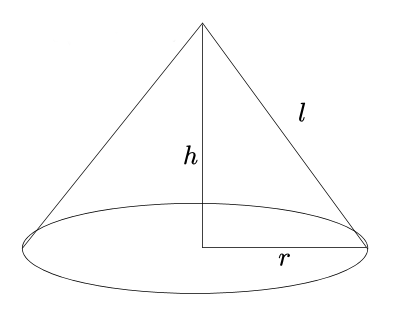
\includegraphics[scale=.35]{lecture3_fig1.png}\\
				
		You are required to design is a cone with a surface area of exactly $25 m^2$ to a tolerance of 0.1 $m^2$ and a height of exactly $1 m$. Your goal is to find the radius in meters.\\

} 


\section{\sectiontitleII}

\frame{
  \frametitle{\sectiontitleII}

	What is the {\it mathematical model} of the cone?  
  
  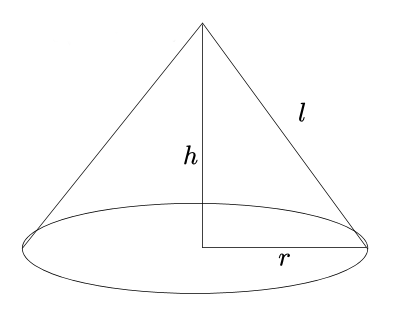
\includegraphics[scale=.35]{lecture3_fig1.png}\\
    \scalebox{1.2}{surface area, $s=\pi r l = \pi r \sqrt{h^2+r^2}$} \\
     \scalebox{1.2}{volume, $v=\pi r^2 \frac{h}{3}$} \\
  	

  
  }

\section{\sectiontitleIII}

\frame{
  \frametitle{\sectiontitleIII}

	How are you going to solve this problem?
	\vspace{50mm}
  
  }
  
  \section{\sectiontitleIV}

\frame{
  \frametitle{\sectiontitleIV}

	How are \underline{you} going to {\it design} the cone? \vspace{5mm}\\
	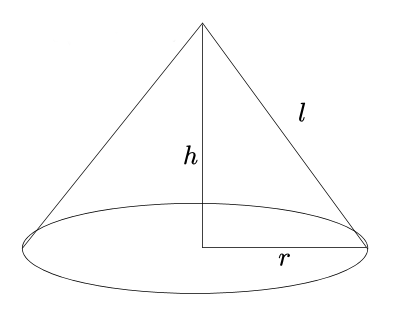
\includegraphics[scale=.35]{lecture3_fig1.png}\\
  
  }



\end{document}

%\begin{document}
%
%\textbf{ \LARGE ME 3001 Lecture - Roots of Non-Linear Equations} \\
%
%\begin{itemize}
%
%
%	\item \textbf{ \LARGE What is a Non-Linear Equation ? }
%			
%			\Large{" an equation whose graph does not form a straight line"} \\ \vspace{20mm}
%
%
%	\item \textbf{ \LARGE Different Types of Non-Linear Equations }
%		
%		\begin{itemize}
%			\item \textbf{\Large Polynomials (excluding first order)} \vspace{30mm}
%			\item \textbf{\Large Transcendentals} \vspace{10mm}
%
%\Large{" a transcendental function "transcends" algebra in that it cannot be expressed in terms of a finite sequence of the algebraic operations of addition, multiplication, and root extraction... "}\\
%				\begin{itemize}
%					\item Exponentials \vspace{10mm}
%					\item Logarithms \vspace{10mm}
%					\item Trigonometrics \vspace{5mm}
%				\end{itemize}
%
%		\end{itemize}
%
%	\item \textbf{ \LARGE What does "Solve the Equation" mean?}
%	\newpage
%
%	\item \textbf{ \LARGE Let us do a simple example} \\\\
%	
%		\hspace{20mm}\scalebox{1.5}{$y = x^2 + 2x - 10$}	 \vspace{80mm}
%		
%		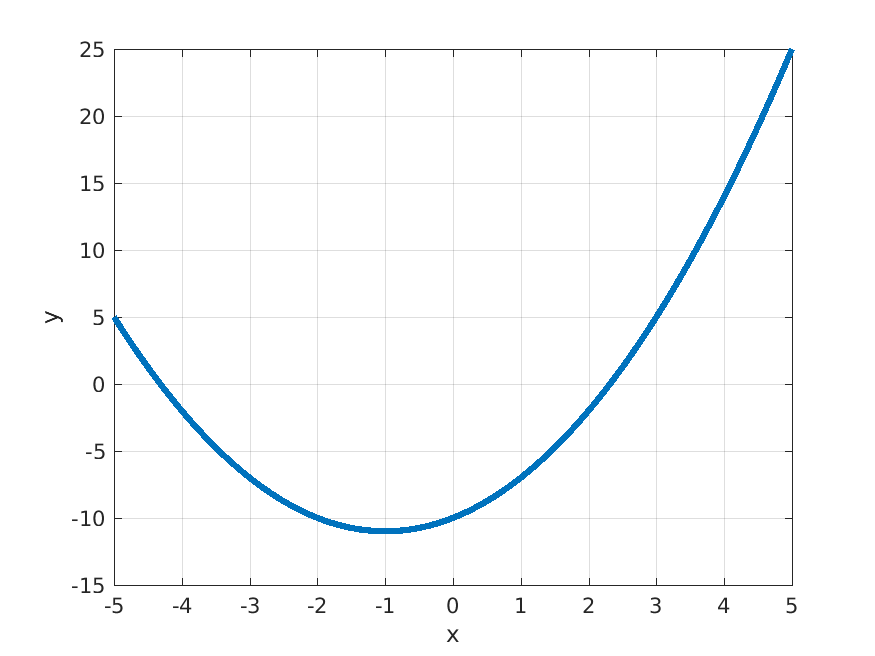
\includegraphics[scale=1]{lecture1_fig1.png}
%		
%		\newpage
%
%
%	\item \textbf{ \LARGE Method 1 - {\it The Incremental Search} }
%
%		
%
%			\begin{itemize}
%			\item \Large{ We are looking for where the line crosses the x-axis, so how can we tell if this happens?} \\ 
%			\item \Large{ Let us investigate with our simple example.} \\ 
%
%			 \hspace{20mm}\scalebox{1.5}{$y = x^2 + 2x - 10$}\vspace{20mm}\\
%		\end{itemize}
%			
\includegraphics[scale=.3]{lecture1_fig4.png}
%			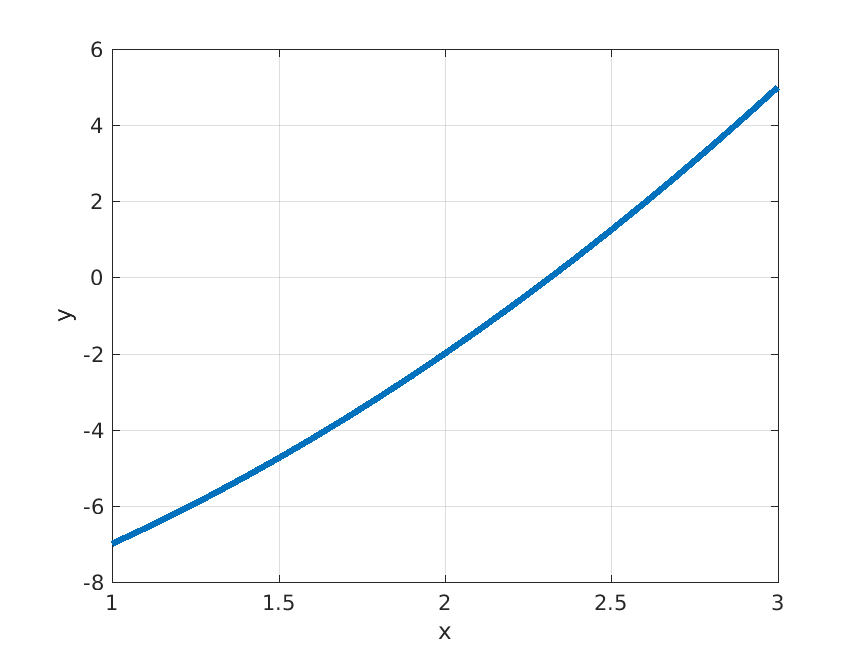
\includegraphics[scale=.8]{lecture1_fig3.png}
%
%		\newpage
%		\item \textbf{ \LARGE Method 2 - {\it The Bisection Method} } \\
%			\begin{itemize}
%				\item different than the previous method because it is a {\it bracketing method}\\
%				\item It is a faster method in general but can you think of any tradeoffs?\\ \vspace{20mm}
%			\end{itemize}
%	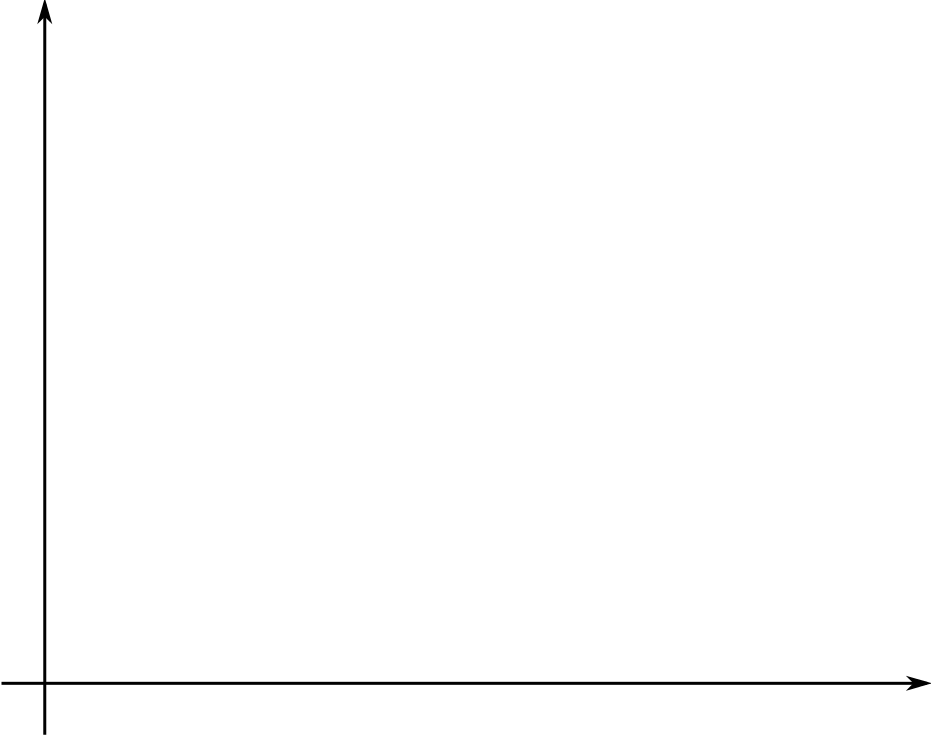
\includegraphics[scale=.5]{lecture1_fig5.png}
%
%	\newpage
%	\item \textbf{ \LARGE {\it Advantages, Disadvantages, and Pitfalls} } \\\\
%	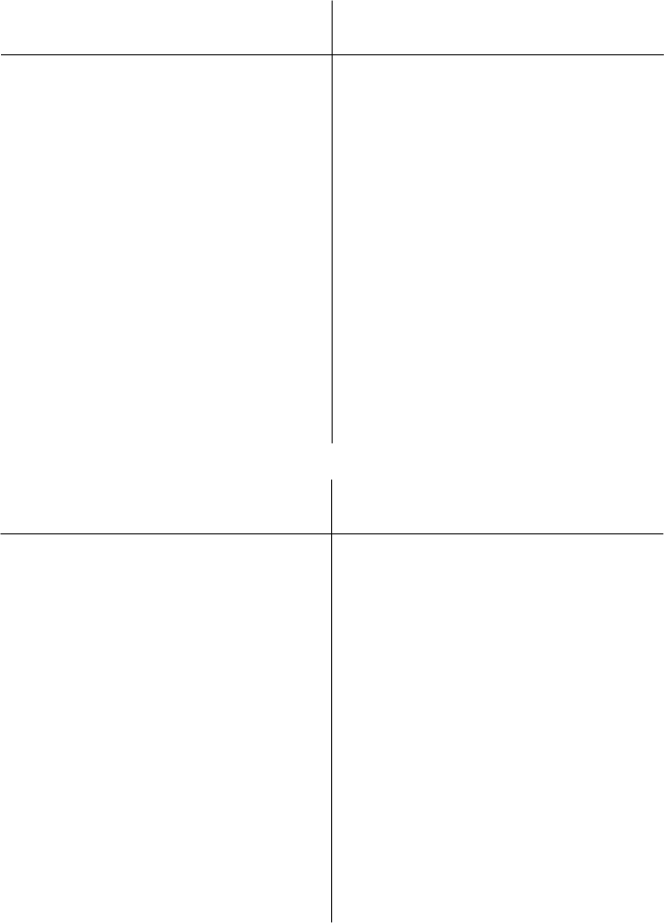
\includegraphics[scale=.65]{lecture1_fig6.png}
%\newpage
%
%	\item \textbf{ \LARGE It is useful to have generalized methods }\\
%		\begin{itemize}
%			\item \Large{A solution technique for the general problem}\\		
%			\item \Large{Standard set of steps or {\it algorithm} for finding the solution}\\\\
%		\end{itemize}
%
%	\item \textbf{ \LARGE The general {\it root-finding} problem }\\\\\\
%	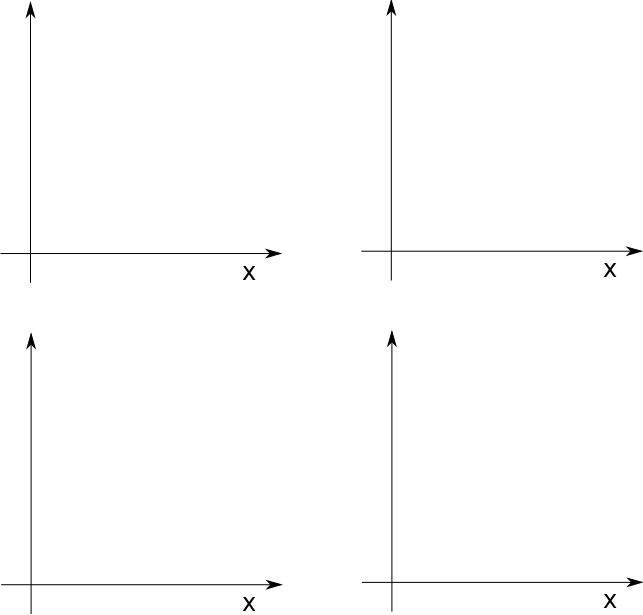
\includegraphics[scale=.6]{lecture1_fig2.png}
%	\newpage 
%
%	\item \textbf{ \LARGE REMINDER - Homework 1 is posted on ilearn } \\
%	
%	 \textbf{ \LARGE DUE: Wednesday, Sep. 5}	\\\\
%
%	\item \textbf{ \LARGE REMINDER - Instructions for Installing MATLAB on your computer have been posted on ilearn. } \\
%	
%
%\end{itemize}
%
%
%	
%
%\end{document}
%
%
%
